\chapter{Hạt, sóng và năng lượng của độ phân giải}

\section{Hạt hay trường?}

Vật lý hạt nghiên cứu điều gì? Hạt---nhưng câu trả lời ấy lập tức làm nảy sinh một câu hỏi cổ xưa. Tự nhiên có rời rạc không? Ở đây, từ này có nghĩa là vật chất tồn tại thành những đơn vị riêng biệt, không thể chia cắt, chứ không phải theo nghĩa kín đáo, khéo ý. Từ Hy Lạp \emph{atom} có nghĩa là không thể chia cắt, dù những vật hiện nay được gọi là nguyên tử vẫn có thể bị tách ra. Tạm thời, \emph{hạt} sẽ là tên gọi chung cho một đơn vị rời rạc.

Bức tranh đối lập là một môi trường liên tục. Khi đó, vật chất không phải là một tập hợp các mảnh riêng rẽ mà là một sự phân bố liên tục trong không gian. Ngôn ngữ tự nhiên của nó là ngôn ngữ của các trường. Một trường là một hàm của vị trí: mật độ của một vật liệu là một trường, và điện trường cùng từ trường cũng là các trường. Các trường sau quyết định các hạt mang điện chuyển động như thế nào, nhưng bản thân chúng, theo quan niệm cổ điển, được phân bố liên tục trong không gian.

Không nên ép thứ tự lịch sử của các ý tưởng này quá mức. Trình tự này hữu ích vì nó phô bày logic của lập luận, chứ không phải vì nó cung cấp một niên biểu đáng tin cậy. Từ vựng của hạt bao gồm nguyên tử, phân tử, va chạm và các vật thể định xứ; từ vựng của tính liên tục bao gồm các trường và các tính chất biến thiên liên tục. Bức tranh nào đúng? Cơ học lượng tử ngăn không cho bức tranh nào hoàn toàn đúng, nhưng cũng ngăn không cho bức tranh nào hoàn toàn sai.

Phần thảo luận này sẽ phần nào tự đủ, dù các lập luận về sau có dựa vào cơ học lượng tử, cơ học cổ điển, thuyết tương đối hẹp và điện từ học. Câu hỏi trước mắt vẫn đơn giản hơn: điều gì đầu tiên đã thuyết phục người ta rằng vật chất thực sự là rời rạc?

\section{Bằng chứng hóa học cho vật chất rời rạc}

Bằng chứng nghiêm túc đầu tiên xuất phát, ít nhất trong cách trình bày logic này, từ hóa học hơn là từ vật lý. Sự phân biệt ấy là giả tạo: hóa học phần lớn là vật lý của nguyên tử và phân tử. Dalton so sánh khối lượng của những số lượng phân tử bằng nhau thuộc các chất khác nhau. Việc xác lập rằng các mẫu chứa số phân tử bằng nhau tự nó đã là một vấn đề lớn. Tên của Avogadro xuất hiện ở đây, và một mol là số Avogadro các phân tử. Giá trị thực của con số đó không cần biết chỉ để so sánh các mẫu chứa cùng số phân tử.

Mẫu hình nổi bật là các khối lượng mol xuất hiện gần đúng như những bội số nguyên của khối lượng mol của hydro. Nói chung, các hệ số nhân không phải là \(3/2\), \(\pi\), hay những số thực tùy ý, mà là những số gần với số nguyên. Carbon-12, chẳng hạn, có khối lượng xấp xỉ bằng mười hai đơn vị khối lượng lấy hydro làm chuẩn. Điều này gợi ý mạnh mẽ rằng chúng được cấu tạo từ những khối xây dựng lặp lại có khối lượng gần như bằng nhau.

Lời giải thích hiện đại loại bỏ điều bí ẩn ấy. Các nguyên tử thông thường chứa proton, neutron và electron. Một electron chỉ có khối lượng khoảng một phần hai nghìn khối lượng của proton hoặc neutron, nên electron đóng góp rất ít vào khối lượng nguyên tử. Proton và neutron mang gần như toàn bộ phần đó, và khối lượng của chúng chênh nhau ít hơn rất nhiều so với một phần trăm. Vì hạt nhân của hydro thông thường là một proton, khối lượng của một nguyên tử hay phân tử xấp xỉ là một bội số nguyên của một khối lượng hạt nhân lấy hydro làm chuẩn. Phát biểu này chỉ gần đúng: khối lượng proton và neutron không đồng nhất, và electron có đóng góp một ít. Tuy vậy, mẫu hình gần nguyên ấy vẫn bộc lộ các thành phần rời rạc.

Khi đó, phân tử được hiểu là những tổ hợp của nguyên tử. Hóa học thế kỷ mười chín nhận diện được khoảng một trăm loại nguyên tử và tổ chức chúng thành các nguyên tố; khoảng chín mươi hai nguyên tố xuất hiện tự nhiên nếu đếm theo nguyên tố, và còn có thêm những phân biệt nữa khi tính cả đồng vị. Bảng tuần hoàn không tuần hoàn theo nghĩa ngây thơ là chỉ đơn giản lặp lại những khối bằng nhau, nhưng nó đã tổ chức các loại riêng biệt ấy. Ở giai đoạn đó, bản thân các nguyên tố có vẻ như là những khối xây dựng cơ bản. Công trình năm 1905 của Einstein đã cung cấp một cách định lượng để xác lập lý thuyết phân tử của vật chất một cách dứt khoát hơn nhiều, nhưng bằng chứng hóa học trước đó đã đủ làm cho bức tranh nguyên tử trở nên thuyết phục.

Gần cuối thế kỷ mười chín, điểm kết thúc tưởng như hiển nhiên này đã không đứng vững. Electron được phát hiện, và phóng xạ bộc lộ những hiện tượng mà bức tranh coi nguyên tố là sơ cấp không thể bao chứa. Bản thân phóng xạ đã chứa, ở quy mô thu nhỏ, nhiều câu hỏi sau này trở thành vật lý hạt nhân và vật lý hạt.

\section{Phóng xạ và các chùm tia tách biệt}

Việc quy công chính xác và niên đại của các sự kiện là điều không chắc chắn. Người ta tạm gắn Becquerel với quan sát rằng vật liệu phóng xạ tình cờ ở gần một bản ảnh và đã tác động lên nó như thể một bức xạ vô hình đã chiếu sáng nó. Thay vì chỉ coi tấm bản ảnh bị ám mờ là hỏng, người ta có thể hỏi điều gì đã tới được nó. Công trình rất rộng về sau của Marie Curie cũng thuộc lịch sử này, nhưng việc phân chia chính xác các khám phá ban đầu không cần thiết cho logic thí nghiệm.

Hãy đặt vật liệu sâu trong một khối chì và chừa một kênh hẹp hướng tới một bản ảnh. Chì hữu ích vì có mật độ lớn, còn kênh hẹp thì chuẩn trực bất cứ thứ gì thoát ra. Thay vì một vệt phơi sáng tản mạn, bản ảnh cho ra một đốm định xứ, gợi ý về một chùm tia có hướng. Theo nghĩa logic này, đó là chùm hạt đầu tiên, dù ở giai đoạn này bản chất của chùm tia chưa được biết.

Bây giờ cho phát xạ đã được chuẩn trực đi qua một từ trường vuông góc với mặt phẳng các quỹ đạo. Vệt phơi sáng tách ra thành ba nhánh. Một nhánh tiếp tục đi thẳng không bị lệch. Hai nhánh cong theo những hướng ngược nhau, và với độ lệch không bằng nhau. Lực từ đổi chiều khi dấu của điện tích đảo, nên các nhánh cong ngược hướng ứng xử như các bức xạ mang điện trái dấu; nhánh đi thẳng ứng xử như bức xạ trung hòa.\footnote{Sơ đồ này tái dựng hình vẽ được xây dựng trong video bài giảng từ 00:14:34 đến 00:19:31.}

\begin{figure}[h]
\centering
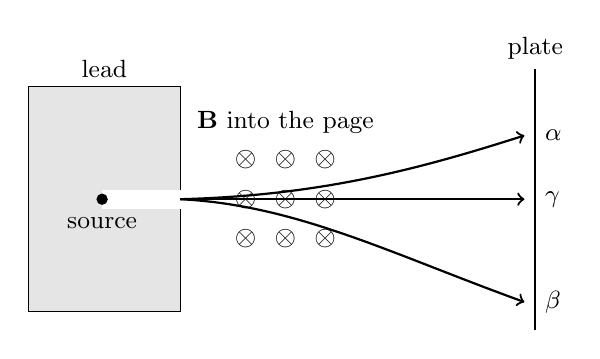
\begin{tikzpicture}[scale=0.92]
\draw[fill=gray!20] (0,-1.55) rectangle (2.1,1.55);
\draw[fill=white,draw=none] (1.02,-0.13) rectangle (2.12,0.13);
\draw[fill=black] (1.02,0) circle (0.07);
\node[below] at (1.02,-0.12) {\small source};
\node[above] at (1.05,1.55) {\small lead};
\foreach \x in {3.0,3.55,4.1}
  \foreach \y in {-0.55,0,0.55}
    \node at (\x,\y) {\(\otimes\)};
\node[above] at (3.55,0.78) {\small \(\mathbf B\) into the page};
\draw[thick] (7,-1.8) -- (7,1.8);
\node[above] at (7,1.8) {\small plate};
\draw[thick,->] (2.1,0) -- (6.85,0);
\draw[thick,->] (2.1,0) .. controls (4.0,0.05) and (5.35,0.40) .. (6.85,0.88);
\draw[thick,->] (2.1,0) .. controls (3.7,-0.08) and (5.0,-0.75) .. (6.85,-1.42);
\node[right] at (7,0.88) {\small \(\alpha\)};
\node[right] at (7,0) {\small \(\gamma\)};
\node[right] at (7,-1.42) {\small \(\beta\)};
\end{tikzpicture}
\caption{Một chùm phóng xạ đã chuẩn trực trong một từ trường ngang. Thành phần trung hòa không bị lệch, còn các thành phần mang điện trái dấu bẻ cong theo những hướng ngược nhau với độ lệch không bằng nhau.}
\end{figure}

Ba thành phần ấy được đặt tên là alpha, beta và gamma. Theo cách nói hiện đại,
\begin{equation}
\begin{aligned}
\beta\text{-radiation} &= \text{electrons},\\
\alpha\text{-radiation} &= \text{helium nuclei},\\
\gamma\text{-radiation} &= \text{photons}.
\end{aligned}
\end{equation}
Một hạt alpha chứa hai proton và hai neutron, giải thích vì sao nó có số khối bằng bốn. Trong dãy gần đúng theo số nguyên của Dalton, vì thế helium sẽ chiếm vị trí số bốn: bốn đơn vị hạt nhân theo thang hydro. Tia beta là các electron mang điện âm đã được biết từ các thí nghiệm tia catốt. Tia gamma không mang điện tích.

Với một nguồn đủ loãng và một đầu dò có khả năng phân giải từng lần đến riêng lẻ, vệt phơi sáng trông liên tục sẽ biến thành một chuỗi sự kiện tách biệt: tách, tách, tách. Điều tương tự có thể thực hiện với bức xạ beta, alpha và gamma. Ống đếm Geiger cho ta đúng bức tranh ấy, dù những thiết bị sớm nhất có được vận hành chính xác trong chế độ đó hay không. Mỗi thành phần đến thành những gói rời rạc. Gamma vẫn là điều gây bối rối: nó trung hòa, thế mà lại được phát hiện từng sự kiện một. Bức xạ gamma là ánh sáng có năng lượng rất cao, và Planck, đặc biệt là Einstein, đã gắn ánh sáng với lượng tử. Tuy nhiên, trước khi đối diện với kết luận đó, phải nghiêm túc xét đến bằng chứng cổ điển rằng ánh sáng là sóng.

\section{Tính chất sóng cổ điển của ánh sáng}

Theo vật lý cổ điển, ánh sáng là ví dụ mạnh mẽ nhất của tính liên tục. Nó gồm các điện trường và từ trường lan truyền dưới dạng sóng liên tục. Newton từng ủng hộ bức tranh tiểu thể, nhưng các thí nghiệm về sóng đã thay thế nó. Làm cho một điện tích dao động sẽ tạo ra bức xạ điện từ. Một ăng-ten vĩ mô có thể phát ra sóng vô tuyến, vi ba, hồng ngoại, ánh sáng khả kiến hoặc tử ngoại; một điện tích chuyển động bên trong nguyên tử cũng là một ăng-ten. Bức xạ phát ra có thể làm lộ sáng một bản ảnh.

Một khe hở đơn cho dấu hiệu đầu tiên của tính chất sóng. Nếu ánh sáng là một dòng đạn, người ta sẽ kỳ vọng một khe nhỏ cho một đốm rất hẹp, được chuẩn trực tốt. Trái lại, vùng sáng loe ra thành một miền mờ. Tuy vậy, chỉ riêng sự loe ra vẫn chưa có tính quyết định, vì người ta có thể hình dung các hạt bị lệch bởi những lực ở rìa của khe.

Hai khe cho phép thử sắc bén hơn. Hai dòng hạt độc lập sẽ cho hai vệt nhòe chồng lên nhau, có lẽ sáng nhất ở nơi chúng chồng lên nhau. Sóng làm điều khác. Một đỉnh sóng từ khe này có thể gặp một đỉnh sóng từ khe kia và tăng cường lẫn nhau; một đỉnh sóng cũng có thể gặp một đáy sóng và triệt tiêu lẫn nhau. Vì thế màn hiện ra các vân sáng và tối xen kẽ, kể cả những chỗ tối mà từng khe đứng riêng đều sẽ chiếu sáng.\footnote{Sơ đồ này tái dựng các hình về khẩu độ và giao thoa được xây dựng trong video bài giảng từ 00:25:00 đến 00:29:49.}

\begin{figure}[h]
\centering
\resizebox{\linewidth}{!}{%
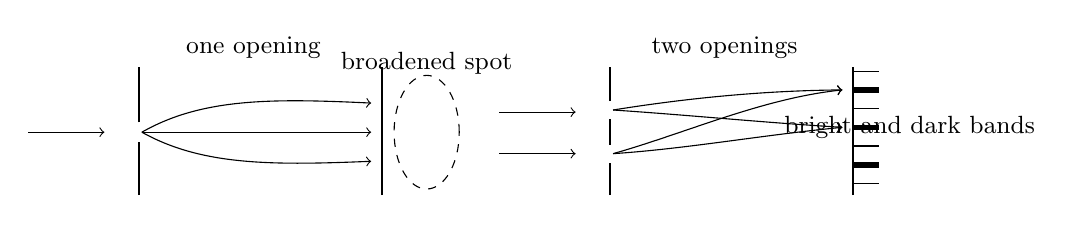
\begin{tikzpicture}[scale=0.88]
\begin{scope}
\draw[->] (-0.3,1.06) -- (0.8,1.06);
\draw[thick] (1.3,0.15) -- (1.3,0.92);
\draw[thick] (1.3,1.20) -- (1.3,2.0);
\draw[thick] (4.8,0.15) -- (4.8,2.0);
\draw[->] (1.34,1.06) .. controls (2.2,1.55) and (3.2,1.55) .. (4.65,1.48);
\draw[->] (1.34,1.06) -- (4.65,1.06);
\draw[->] (1.34,1.06) .. controls (2.2,0.58) and (3.2,0.58) .. (4.65,0.64);
\draw[dashed] (5.45,1.06) ellipse (0.47 and 0.82);
\node at (2.95,2.28) {\small one opening};
\node at (5.45,2.05) {\small broadened spot};
\end{scope}
\begin{scope}[xshift=6.8cm]
\draw[->] (-0.3,1.35) -- (0.8,1.35);
\draw[->] (-0.3,0.75) -- (0.8,0.75);
\draw[thick] (1.3,0.15) -- (1.3,0.62);
\draw[thick] (1.3,0.88) -- (1.3,1.25);
\draw[thick] (1.3,1.51) -- (1.3,2.0);
\draw[thick] (4.8,0.15) -- (4.8,2.0);
\draw[thin] (4.8,0.32) -- (5.18,0.32);
\draw[line width=2pt] (4.8,0.59) -- (5.18,0.59);
\draw[thin] (4.8,0.86) -- (5.18,0.86);
\draw[line width=2pt] (4.8,1.13) -- (5.18,1.13);
\draw[thin] (4.8,1.40) -- (5.18,1.40);
\draw[line width=2pt] (4.8,1.67) -- (5.18,1.67);
\draw[thin] (4.8,1.94) -- (5.18,1.94);
\draw[->] (1.34,0.75) .. controls (2.4,0.82) and (3.5,1.02) .. (4.65,1.13);
\draw[->] (1.34,1.38) .. controls (2.4,1.31) and (3.5,1.20) .. (4.65,1.13);
\draw[->] (1.34,0.75) .. controls (2.4,1.05) and (3.5,1.55) .. (4.65,1.67);
\draw[->] (1.34,1.38) .. controls (2.4,1.55) and (3.5,1.66) .. (4.65,1.67);
\node at (2.95,2.28) {\small two openings};
\node at (5.62,1.13) {\small bright and dark bands};
\end{scope}
\end{tikzpicture}
}
\caption{Một khẩu độ đơn tạo ra một ảnh mở rộng, còn hai khẩu độ tạo ra các vân sáng tối xen kẽ do giao thoa tăng cường và triệt tiêu.}
\end{figure}

Hiệu ứng tương tự rất dễ hình dung với nước. Hãy lắc hai ngón tay trên mặt nước: các sóng tròn lan ra, tăng cường ở một số nơi và triệt tiêu ở những nơi khác. Chính giao thoa, chứ không chỉ sự lan rộng đơn thuần, mới là dấu hiệu quyết định của sóng.

Trình tự lịch sử ở đây một lần nữa không hề đơn giản. Trong cách kể mang tính sơ đồ này, Huygens được đặt trước Newton như một người chủ trương sự lan truyền dạng sóng; Thomas Young gắn với minh chứng về giao thoa; và một số thí nghiệm quang học của chính Newton cũng cho phép một cách diễn giải theo giao thoa sóng dù ông ưa chuộng tiểu thể. Các thí nghiệm giao thoa về sau đã xác lập tính chất sóng của ánh sáng vượt quá mọi nghi ngờ hợp lý.

Maxwell sau đó đã xác định cái gì dao động. Nếu một sóng ánh sáng truyền dọc theo một trục, điện trường của nó vuông góc với trục ấy. Từ trường của nó cũng vuông góc với trục truyền và vuông góc với điện trường. Toàn bộ mẫu hình ấy truyền đi với tốc độ ánh sáng.\footnote{Sơ đồ này tái dựng hình sóng điện từ được vẽ trong video bài giảng tại 00:31:08.}

\begin{figure}[h]
\centering
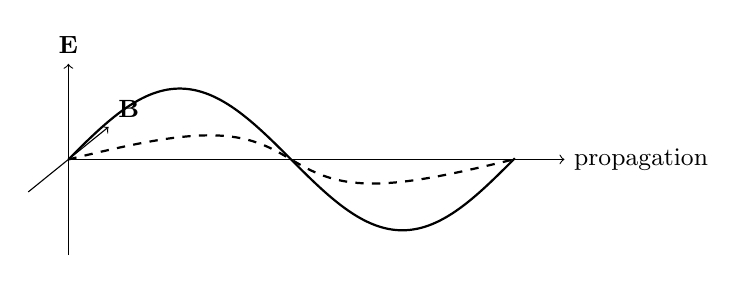
\begin{tikzpicture}[
  scale=0.9,
  x={(1cm,0cm)},
  y={(0cm,1cm)},
  z={(0.42cm,0.34cm)}
]
\draw[->] (0,0,0) -- (7,0,0) node[right] {\small propagation};
\draw[->] (0,-1.35,0) -- (0,1.35,0) node[above] {\small \(\mathbf E\)};
\draw[->] (0,0,-1.35) -- (0,0,1.35) node[above right] {\small \(\mathbf B\)};
\draw[thick,smooth,variable=\x,domain=0:6.3,samples=100]
  plot ({\x},{sin(\x r)},0);
\draw[thick,dashed,smooth,variable=\x,domain=0:6.3,samples=100]
  plot ({\x},0,{sin(\x r)});
\end{tikzpicture}
\caption{Trong sóng điện từ, điện trường và từ trường vuông góc với nhau, và cả hai đều vuông góc với hướng truyền.}
\end{figure}

Ánh sáng khả kiến thông thường dao động quá nhanh để có thể theo dõi trực tiếp các trường luân phiên ấy. Đối với một sóng vô tuyến cực dài, dao động sẽ chậm đi tương ứng. Trong cả hai trường hợp, cùng một hình học sóng ngang ấy tạo ra giao thoa.

\section{Bước sóng, chu kỳ và tần số}

Bước sóng \(\lambda\) là một khoảng cách trong không gian: bắt đầu ở một điểm nào đó của dao động rồi đi dọc theo sóng cho tới khi cùng một pha lặp lại sau một chu trình trọn vẹn. Nó được đo bằng mét, xentimét, hay bất kỳ đơn vị độ dài nào khác.

Bây giờ hãy đứng yên tại một vị trí trong khi sóng đi qua. Thời gian cần cho một chu trình trọn vẹn là chu kỳ \(T\). Ánh sáng khả kiến có chu kỳ cực ngắn, xấp xỉ cỡ \(10^{-15}\,\mathrm{s}\); bước sóng dài hơn tương ứng với chu kỳ dài hơn, và bước sóng ngắn hơn tương ứng với chu kỳ ngắn hơn.

Trong một chu kỳ, sóng tiến đi đúng một bước sóng, nên một sóng có tốc độ \(v\) tuân theo
\begin{equation}
v=\frac{\lambda}{T}.
\end{equation}
Sóng nước và sóng âm có các tốc độ truyền riêng của chúng. Đối với ánh sáng,
\begin{equation}
c=\frac{\lambda}{T}.
\end{equation}
Tần số \(f\) là số chu trình trong một đơn vị thời gian:
\begin{equation}
f=\frac{1}{T}.
\end{equation}
Do đó
\begin{equation}
\lambda f=c.
\end{equation}
Biết bước sóng hay tần số đều xác định được đại lượng kia.

\begin{figure}[h]
\centering
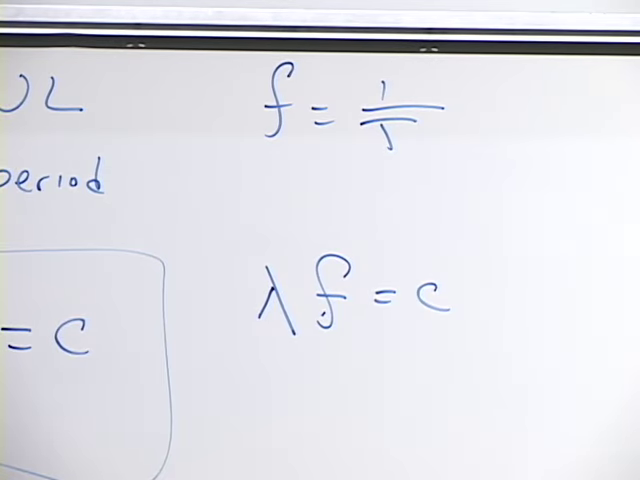
\includegraphics[width=0.68\textwidth]{lecture_01_figure_03.png}
\caption{Đối với sóng ánh sáng, \(f=1/T\) và \(\lambda f=c\).}
\lectureframe{00:36:24}
\end{figure}

Các nhà vật lý thường đo tốc độ dao động bằng radian trên giây thay vì bằng số chu kỳ trọn vẹn trên giây. Hãy hình dung chuyển động đều trên một đường tròn. Nếu điểm đó hoàn thành \(f\) vòng mỗi giây và mỗi vòng chứa \(2\pi\) radian, thì tần số góc của nó là
\begin{equation}
\omega=2\pi f,
\qquad
\frac{\omega}{2\pi}=f.
\end{equation}
Hiện giờ đây chỉ là một định nghĩa; câu hỏi thực hành rằng liệu nó có làm giảm số lượng các thừa số \(2\pi\) hay không sẽ quay lại sau.

Kết hợp \(f=c/\lambda\) với \(\omega=2\pi f\) ta được
\begin{equation}
\omega=\frac{2\pi c}{\lambda},
\qquad
\omega\lambda=2\pi c.
\end{equation}
Đối với một loại sóng khác, thay \(c\) bằng tốc độ lan truyền của sóng đó.

\begin{figure}[h]
\centering
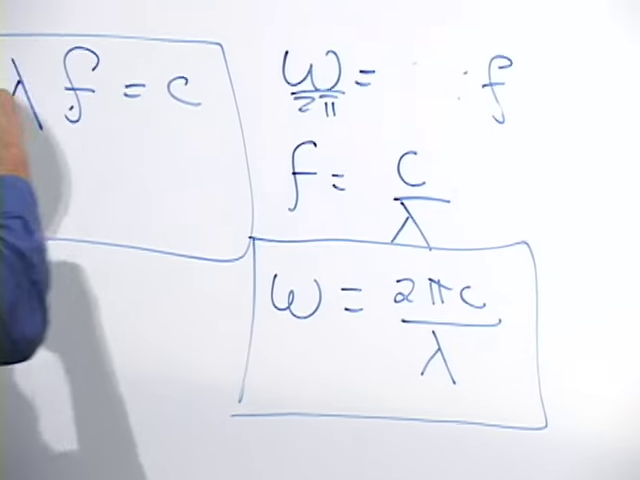
\includegraphics[width=0.68\textwidth]{lecture_01_figure_04.png}
\caption{Với \(\omega=2\pi f\), sóng ánh sáng thỏa mãn \(\omega=2\pi c/\lambda\).}
\lectureframe{00:39:10}
\end{figure}

Bức xạ điện từ tạo thành một phổ liên tục. Sắp theo thứ tự từ bước sóng dài hơn đến ngắn hơn, các tên gọi quy ước là
\begin{equation}
\begin{aligned}
\text{radio}
&\longrightarrow \text{microwave}
\longrightarrow \text{infrared}
\longrightarrow \text{visible}\\
&\longrightarrow \text{ultraviolet}
\longrightarrow \text{X ray}
\longrightarrow \text{gamma ray}.
\end{aligned}
\end{equation}
Ánh sáng khả kiến chỉ chiếm một khoảng hẹp. Ranh giới giữa các vùng được đặt tên là có tính quy ước, nên ở đây không cần các bước sóng phân chia chính xác. Sóng vô tuyến có thể cực kỳ dài; bức xạ gamma là đầu bước sóng rất ngắn của phổ điện từ. Khó khăn giờ đây trở nên sắc nét: bức xạ gamma về mặt cổ điển là một sóng trường liên tục, thế nhưng nó lại được phát hiện dưới dạng các tín hiệu rời rạc.

\section{Các lần đến rời rạc và xác suất do sóng chi phối}

Các tính chất nhiệt động lực học của bức xạ đã dẫn Planck và Einstein đến kết luận rằng ánh sáng phải được xử lý theo các đơn vị rời rạc. Một thí nghiệm tưởng tượng làm cho điểm này trở nên sinh động, nhưng đó không phải là một khẳng định về con đường lịch sử thực sự dẫn đến phát hiện ấy.

Chiếu một chùm tia lên một màn. Ở cường độ thông thường, nó tạo thành một đốm sáng trông như liên tục. Đặt một bộ suy giảm bán đục vào chùm tia: đốm sáng trở nên mờ hơn. Tăng độ suy giảm lặp đi lặp lại thì lượng ánh sáng đến trong mỗi đơn vị thời gian giảm đi. Cuối cùng, hình ảnh thay đổi. Thay vì một đốm mờ liên tục, bộ dò ghi nhận các sự kiện tách biệt.\footnote{Sơ đồ này tái dựng thí nghiệm suy giảm được triển khai trong video bài giảng trong khoảng từ 00:42:32 đến 00:45:42.}

\begin{figure}[h]
\centering
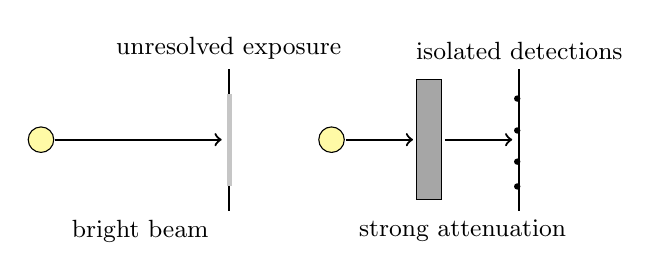
\begin{tikzpicture}[scale=0.9]
\begin{scope}
\draw[fill=yellow!35] (0,0) circle (0.18);
\draw[->,thick] (0.2,0) -- (2.55,0);
\draw[thick] (2.65,-1.0) -- (2.65,1.0);
\node[below] at (1.4,-1.0) {\small bright beam};
\end{scope}
\begin{scope}[xshift=4.1cm]
\draw[fill=yellow!35] (0,0) circle (0.18);
\draw[->,thick] (0.2,0) -- (1.15,0);
\draw[fill=gray!70] (1.2,-0.85) rectangle (1.55,0.85);
\draw[->,thick] (1.6,0) -- (2.55,0);
\draw[thick] (2.65,-1.0) -- (2.65,1.0);
\node[below] at (1.85,-1.0) {\small strong attenuation};
\end{scope}
\fill[gray!45] (2.62,-0.65) rectangle (2.70,0.65);
\foreach \y in {-0.66,-0.31,0.13,0.58}
  \fill (6.72,\y) circle (0.045);
\node[above] at (2.65,1.0) {\small unresolved exposure};
\node[above] at (6.75,1.0) {\small isolated detections};
\end{tikzpicture}
\caption{Sự suy giảm tăng dần làm giảm tốc độ phát hiện cho đến khi một ảnh phơi sáng trông như liên tục được phân giải thành các sự kiện photon riêng lẻ.}
\end{figure}

Chờ đủ lâu thì những sự kiện ấy tích lũy thành cùng một dạng phân bố không gian như đốm ban đầu. Vì vậy, vùng sáng là tổng chưa được phân giải của nhiều lần đến riêng lẻ. Thí nghiệm cường độ thấp này có thể thực hiện được, dù nó không phải là thí nghiệm thời kỳ đầu đã ban đầu thúc đẩy giả thuyết photon. Đề xuất photon của Einstein nảy sinh từ những xem xét nhiệt động lực học và quang điện; thí nghiệm suy giảm cung cấp một cách đặc biệt trực tiếp để hình dung hệ quả của nó.

Bây giờ hãy đặt hai lỗ mở trong chùm tia và giảm cường độ cho đến khi các photon đến từng cái một. Mỗi lần phát hiện là một vết chấm cục bộ. Thế nhưng sau nhiều lần phát hiện, các vết chấm ấy lấp đầy một hình giao thoa, gồm cả các vân sáng và tối. Các lần đến rời rạc là ngẫu nhiên, nhưng phân bố xác suất của chúng chính là phân bố do hình sóng dự đoán. Sóng cổ điển đã trở thành một sóng chi phối các xác suất.

Vì vậy, sóng và hạt không phải là hai loại thực thể tách biệt được gán cho những phần khác nhau của tự nhiên. Chúng là hai biểu hiện của cùng một đối tượng lượng tử. Không thể mô tả đầy đủ ánh sáng chỉ như sóng hoặc chỉ như hạt.

Electron đảo ngược điều ngạc nhiên ban đầu. Electron được chấp nhận là hạt và đến bộ dò từng cái một, nhưng với các lỗ mở đủ gần nhau chúng cũng tạo nên một hình giao thoa. Hạt alpha, nặng hơn electron khoảng 8000 lần, tuân theo cùng nguyên lý đó, mặc dù thí nghiệm khó hơn. Giao thoa thậm chí còn đã được quan sát với buckyball: các phân tử gồm 60 nguyên tử carbon được sắp xếp xấp xỉ như một dạng tổng quát của quả bóng đá. Nguyên lý ấy được kỳ vọng là áp dụng ngay cả cho các quả bóng bowling, mặc dù một thí nghiệm như vậy là cực kỳ bất khả thi về mặt thực hành. Có thể đẩy thảo luận xa hơn tới các thí nghiệm được đề xuất với virus hoặc tế bào sống như những ví dụ ngày càng táo bạo hơn. Hiểu được mô tả sóng và mô tả hạt ăn khớp với nhau như thế nào đòi hỏi cơ học lượng tử; nhiệm vụ trước mắt là rút ra các tính chất của photon cần cho vật lý hạt.

\section{Năng lượng photon}

Photon là những thành phần rời rạc, không thể chia của ánh sáng. Ánh sáng mang năng lượng---ánh sáng mặt trời làm nóng một vật hấp thụ---nên mỗi photon phải mang năng lượng. Một sóng đơn sắc có bước sóng và tần số góc xác định, và mỗi photon trong đó có
\begin{equation}
E_\gamma=\hbar\omega.
\end{equation}
Cố hình dung một sóng liên tục như một tập hợp cơ học gồm những chấm nhỏ là gây hiểu lầm. Điều xác định là sự kết hợp thực nghiệm sau: các phát hiện cục bộ xảy ra theo một phân bố do sóng chi phối, và năng lượng đến theo những đơn vị không thể chia.

Vì
\begin{equation}
\omega=\frac{2\pi c}{\lambda},
\end{equation}
một bước sóng ngắn hơn có nghĩa là một tần số góc lớn hơn và do đó nhiều năng lượng hơn trong mỗi photon:
\begin{equation}
\lambda\downarrow
\quad\Longrightarrow\quad
\omega\uparrow
\quad\Longrightarrow\quad
E_\gamma\uparrow.
\end{equation}
Một photon vô tuyến đơn lẻ có rất ít năng lượng. Tuy nhiên, một chùm vô tuyến vẫn có thể mang tổng năng lượng khổng lồ bằng cách chứa rất nhiều photon. Đối với một xung đơn sắc chứa \(n\) photon,
\begin{equation}
E_{\text{pulse}}=n\hbar\omega,
\qquad
n=0,1,2,\ldots.
\end{equation}
Tổng năng lượng có thể lớn, nhưng nó vẫn là một bội số nguyên của năng lượng một photon.

Hệ thức này dẫn tới câu hỏi thực tiễn sẽ chi phối phần còn lại của cuộc thảo luận. Tại sao phải xây những cỗ máy ngày càng lớn hơn để nhìn thấy những thứ ngày càng nhỏ hơn? Tại sao không dùng một cỗ máy nhỏ cho một vật nhỏ? Nửa đầu của câu trả lời đã có sẵn: phân giải cấu trúc nhỏ hơn đòi hỏi bước sóng ngắn hơn, và một lượng tử có bước sóng ngắn hơn mang năng lượng lớn hơn.

\section{Năng lượng nghỉ và khối lượng bất biến}

Vật lý hạt kết hợp cơ học lượng tử với thuyết tương đối. Hệ thức photon \(E_\gamma=\hbar\omega\) cung cấp phía lượng tử; sự kiện sơ đẳng tương ứng từ thuyết tương đối là
\begin{equation}
E_{\mathrm{rest}}=mc^2.
\end{equation}
Điều kiện kèm theo này rất quan trọng. Các trình bày cũ phân biệt \emph{khối lượng nghỉ} với \emph{khối lượng chuyển động} phụ thuộc vận tốc. Thuật ngữ hiện đại dùng \emph{khối lượng} để chỉ khối lượng bất biến của một vật. Chuyển động làm thay đổi năng lượng của nó, chứ không làm thay đổi khối lượng của nó. Mọi electron đều có cùng một khối lượng, bất kể trạng thái chuyển động của nó ra sao, trong khi năng lượng của electron tăng lên khi nó được gia tốc. Vì vậy, \(E=mc^2\), ở dạng này, là năng lượng của một vật có khối lượng trong một hệ quy chiếu mà toàn bộ vật đứng yên.

Vật không nhất thiết phải không có chuyển động nội tại. Một hộp khí có thể đứng yên trên cân trong khi các phân tử của nó chuyển động nhanh theo mọi hướng. Năng lượng của những chuyển động nội tại ấy là một phần của năng lượng nghỉ của toàn bộ chiếc hộp. Hãy bắt đầu với một chiếc hộp lạnh, đo khối lượng của nó, rồi thêm nhiệt năng trong khi vẫn giữ chính chiếc hộp đứng yên. Khối lượng nghỉ của nó thay đổi một lượng
\begin{equation}
\Delta m=\frac{\Delta E_{\mathrm{internal}}}{c^2}.
\end{equation}
Trọng lượng và quán tính của nó tăng cùng với khối lượng. Đối với một chiếc hộp thông thường, ngay cả sau khi nhiệt độ tăng nhiều, hiệu ứng ấy vẫn quá nhỏ để nhận ra trên một cái cân thông thường; độ nhỏ của hiệu ứng không làm thay đổi nguyên lý.

Một ví dụ sắc nét hơn xét một electron và một positron. Chúng có khối lượng bằng nhau chính xác và điện tích trái dấu. Nếu ban đầu chúng đứng yên và hủy nhau, các photon mang năng lượng đi:
\begin{equation}
e^-+e^+\longrightarrow \text{photons}.
\end{equation}
Năng lượng ban đầu là
\begin{equation}
E_{\mathrm{initial}}=2m_e c^2,
\end{equation}
và năng lượng đó không thể biến mất. Một cặp đơn lẻ chỉ cho một lượng cực nhỏ, nên cần một số lượng cặp khổng lồ mới có thể đun nóng dù chỉ một cốc cà phê, nhưng các sự kiện hủy riêng lẻ cho thấy trực tiếp sự chuyển đổi ấy.

Vì vậy, đối với một vật đứng yên, khối lượng và năng lượng là cùng một đại lượng vật lý được biểu diễn bằng các đơn vị khác nhau. Hệ số \(c^2\) là hệ số chuyển đổi giữa các đơn vị khối lượng và năng lượng thông dụng, cũng như một hệ số số học chuyển mét thành xentimét.

\begin{classroomqa}
\lecturetimestamp{01:04:39}
\audiencequestion{Việc chuyển khối lượng thành năng lượng được giải phóng có đòi hỏi một cơ chế không?}
\lecturerresponse{Có, cần một cơ chế vật lý, nhưng các định luật bảo toàn đã ràng buộc kết quả của nó. Ngay cả trước khi mô tả cơ chế hủy vi mô, năng lượng ban đầu của cặp electron--positron vẫn phải xuất hiện lại ở đâu đó. Vì vậy, bảo toàn năng lượng có thể quyết định một phần quan trọng của câu trả lời mà không cần trình bày chi tiết về tương tác.}
\end{classroomqa}

\section{Thứ nguyên và việc chọn đơn vị}

Trong hệ đơn vị SI, tốc độ ánh sáng là một số rất lớn và hằng số Planck là một số rất nhỏ. Độ nhỏ của đại lượng sau đã được gợi ra ngay bởi hệ thức photon: tần số góc của ánh sáng khả kiến là cực lớn trong khi năng lượng của một photon thì cực nhỏ, nên \(E_\gamma=\hbar\omega\) đòi hỏi \(\hbar\) phải có một giá trị số nhỏ trong các đơn vị này. Xét theo bậc độ lớn,
\begin{equation}
c\sim 10^8\ \mathrm{m\,s^{-1}},
\qquad
\hbar\sim 10^{-34}\ \mathrm{J\,s}.
\end{equation}
\editorialnote{Chỉ giữ lại các bậc độ lớn đã nêu trong bài giảng vì các chữ số cuối trên bảng không rõ.}
Các đơn vị là thiết yếu: không hằng số nào trong hai hằng số này chỉ đơn thuần là một số thập phân. Vì năng lượng có thứ nguyên
\begin{equation}
[E]=M L^2 T^{-2},
\end{equation}
và \(E_\gamma=\hbar\omega\) với \([\omega]=T^{-1}\), nên hằng số Planck có thứ nguyên
\begin{equation}
[\hbar]=[E]T=M L^2 T^{-1}.
\end{equation}

Việc gọi \(c\) là lớn và \(\hbar\) là nhỏ đã ngầm giả định một lựa chọn đơn vị. Đo tốc độ bằng foot trên giờ cho giá trị số của \(c\) khác với khi đo bằng mét trên giây. Tính theo năm ánh sáng trên năm, hoặc giây ánh sáng trên giây, tốc độ ánh sáng đơn giản là một. Tương tự, một lựa chọn phối hợp thích hợp của các đơn vị khối lượng, độ dài và thời gian cũng có thể làm cho \(\hbar=1\).

Các hệ đơn vị quen thuộc là những quy ước được thừa hưởng, không phải những đặc trưng được tự nhiên ưu đãi. Một dặm có 5280 foot, một stone có 14 pao, ngựa được đo bằng gang tay, và công suất có thể được đo bằng mã lực. Các đơn vị mét là có hệ thống hơn, nhưng thang của chúng vẫn là những lựa chọn của con người. Không có gì trong vật lý cơ bản khiến mét, giây hay kilôgam trở thành đơn vị đặc biệt.

Độ dài, thời gian và khối lượng cung cấp 3 lựa chọn đơn vị cơ bản độc lập:
\begin{equation}
L,\qquad T,\qquad M.
\end{equation}
Các đơn vị cơ học khác có thể được xây dựng từ chúng. Những lựa chọn hữu ích phụ thuộc vào bài toán. Một khối lượng Mặt Trời là thuận tiện trong vật lý thiên văn; một khối lượng proton có thể thuận tiện trong vật lý hạt nhân; năm ánh sáng và năm làm cho các công thức thiên văn tương đối tính trở nên gọn hơn. Với 3 lựa chọn độc lập, người ta có thể gán các giá trị số thuận tiện cho 3 hằng số có thứ nguyên độc lập. Vật lý thiên văn, vật lý nguyên tử và vật lý hạt không nhất thiết phải dùng cùng những lựa chọn đó.

Đối với vật lý hạt, 2 quy ước đặc biệt hữu ích là
\begin{equation}
c=1,
\qquad
\hbar=1.
\end{equation}
Không có một khối lượng hạt nào nổi bật tương đương cho đơn vị còn lại. Người ta có thể tuyên bố khối lượng proton, khối lượng boson Higgs hoặc khối lượng muon bằng một, nhưng như thế chỉ đơn thuần ưu ái một thành viên trong một tập hợp lớn.

Vậy tại sao lại chọn \(c\) và \(\hbar\)? Một câu trả lời đầu tiên có thể là chúng xuất hiện trong nhiều phương trình. Chỉ tần suất xuất hiện thì chưa đủ: khối lượng proton cũng xuất hiện trong nhiều phương trình, kích thước của proton cũng vậy. Điều làm \(c\) và \(\hbar\) khác biệt là tính phổ quát của chúng.

Các hằng số \(c\) và \(\hbar\) là khác loại. Tốc độ \(c\) ràng buộc mọi vật thể vật lý: các vật có khối lượng có thể tiến gần tới nó nhưng không thể được gia tốc để vượt qua nó. Hằng số Planck ràng buộc mọi đối tượng lượng tử thông qua hệ thức bất định theo bậc độ lớn
\begin{equation}
\Delta x\,\Delta p\gtrsim\hbar.
\end{equation}
Không phát biểu nào trong hai phát biểu ấy đặc cách một loại hạt cụ thể. Chính tính phổ quát này làm cho \(c=1\) và \(\hbar=1\) trở thành những quy ước tự nhiên.

Proton không cung cấp một thang chuẩn phổ quát tương đương. Nó chỉ là một vật trong rất nhiều vật. Đặt khối lượng proton bằng một không có địa vị cơ bản hơn gì việc đặt khối lượng của một nguyên tử rubidi bằng một; electron, boson Higgs và muon cũng gặp cùng khó khăn ấy.

Điện tích gợi ý một đại lượng phổ quát khác, nhưng sau khi \(c\) và \(\hbar\) đã được chuẩn hóa, hằng số ghép điện từ có ý nghĩa vật lý là vô thứ nguyên. Thay đổi đơn vị có thể dịch chuyển các hằng số có thứ nguyên qua lại trong một công thức điện từ; nó không thể thay đổi một hằng số ghép vô thứ nguyên thực sự.

Hấp dẫn cung cấp một hằng số phổ quát có thứ nguyên. Dưới dạng Newton, độ lớn của lực giữa hai khối lượng là
\begin{equation}
F=G\frac{m_1m_2}{r^2}.
\end{equation}
Mọi khối lượng đều hấp dẫn, trong khi các vật trung hòa điện không nhất thiết tham gia vào một lực điện. Vì vậy \(G\) có tính phổ quát cần thiết. Tuy nhiên, nó là một chuẩn hóa thực tiễn kém cho vật lý hạt thông thường, vì các lực hấp dẫn giữa những hạt cơ bản đã biết là không đáng kể trong các phép tính đang được bàn tới.

\begin{classroomqa}
\lecturetimestamp{01:20:34}
\audiencequestion{Có hợp lệ không nếu đơn giản gạt bỏ \(G\)? Ở năng lượng rất cao, các hạt cơ bản có thể không tuân theo hấp dẫn cổ điển theo cách đang được giả định.}
\lecturerresponse{Từng hạt riêng lẻ quả thực có phản ứng với trường hấp dẫn của Trái Đất: một hạt đơn lẻ rơi trong trường đó. Ảnh hưởng hấp dẫn của một hạt cơ bản này lên một hạt cơ bản khác chưa được đo trực tiếp, nên giả định về tính phổ quát có thể bị đặt dấu hỏi ở cấp độ ấy. Lý do trực tiếp để bỏ \(G\) ra ngoài mang tính thực tiễn hơn là tuyệt đối: hấp dẫn đóng góp không đáng kể vào các thí nghiệm và phương trình vật lý hạt thông thường.}
\end{classroomqa}

\begin{classroomqa}
\lecturetimestamp{01:22:01}
\audiencequestion{Liệu tương tác điện có thể được dùng làm quy ước ấn định đơn vị thứ ba thay cho hấp dẫn không?}
\lecturerresponse{Có. Ta có thể chọn các đơn vị điện từ trong đó điện tích, hoặc hằng số xuất hiện trong định luật Coulomb, được chuẩn hóa. Những quy ước như vậy quả có được sử dụng. Electron đẩy nhau chứ không hút nhau, nhưng dấu đó không cản trở lựa chọn này. Chỉ là đây không phải quy ước được dùng ở đây.}
\end{classroomqa}

\begin{classroomqa}
\lecturetimestamp{01:23:06}
\audiencequestion{Một khi \(c\) và \(\hbar\) được đặt bằng 1, điện tích có phải là vô thứ nguyên không?}
\lecturerresponse{Có. Một đại lượng vô thứ nguyên gắn với bình phương điện tích điện có giá trị xấp xỉ \(1/137\). Quy ước chính xác và ý nghĩa của con số đó có thể để lại bàn sau; điểm ở đây là nó vô thứ nguyên.}
\end{classroomqa}

\begin{classroomqa}
\lecturetimestamp{01:23:37}
\audiencequestion{Có thể chọn hằng số Coulomb làm hằng số thứ ba được đặt bằng 1 không?}
\lecturerresponse{Nó có thể được hấp thụ vào quy ước đơn vị điện từ. Lựa chọn đó không thể biến hằng ghép vô thứ nguyên \(1/137\) thành 1, vì đổi đơn vị không thể làm thay đổi một số vô thứ nguyên. Ở đây không khẳng định có lợi ích đặc biệt nào khi dùng quy ước đó.}
\end{classroomqa}

\section{Các phương trình trong đơn vị tự nhiên và các hệ quy chiếu}

Khi \(c=1\), hệ thức năng lượng nghỉ đối với một vật có khối lượng trở thành
\begin{equation}
E_{\mathrm{rest}}=m.
\end{equation}
Khi \(\hbar=1\), hệ thức cho photon trở thành
\begin{equation}
E_\gamma=\omega.
\end{equation}
Có thể khôi phục các hằng số bất cứ khi nào cần đến các giá trị số trong những đơn vị thông thường.

\begin{figure}[h]
\centering
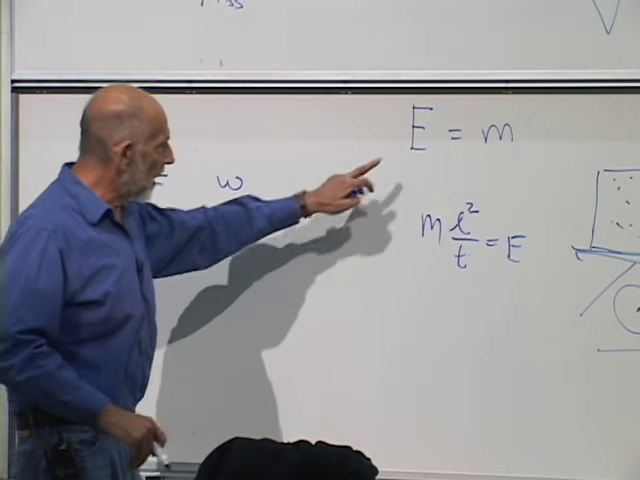
\includegraphics[width=0.72\textwidth]{lecture_01_figure_05.png}
\caption{Trong hệ đơn vị với \(c=1\), năng lượng nghỉ của một vật có khối lượng đứng yên là \(E=m\).}
\lectureframe{01:25:40}
\end{figure}

Những công thức này trông giống nhau nhưng mang ý nghĩa khác nhau. Trong \(E_{\mathrm{rest}}=m\), \(E\) là năng lượng nghỉ của một vật có khối lượng. Photon không có khối lượng và không thể được đưa về trạng thái nghỉ, nên năng lượng của nó không phải là năng lượng nghỉ. Hệ thức \(E_\gamma=\omega\) cho năng lượng của một lượng tử không khối lượng đang chuyển động.

\begin{classroomqa}
\lecturetimestamp{01:26:07}
\audiencequestion{\emph{đứng yên} có nghĩa là gì khi trạng thái nghỉ luôn là tương đối đối với một cái gì đó và bản thân phòng thí nghiệm cũng không tuyệt đối đứng yên?}
\lecturerresponse{Trạng thái nghỉ được định nghĩa tương đối với một hệ quy chiếu được chọn. Nếu một cái cốc đứng yên so với phòng thí nghiệm, thì trong hệ quy chiếu của phòng thí nghiệm đó, năng lượng của nó bằng khối lượng của nó khi \(c=1\), không có đóng góp động năng tổng thể nào. Một quan sát viên khác chuyển động ngang qua cái cốc sẽ gán cho nó cả động năng nữa. Nói chung, các quan sát viên khác nhau sẽ gán những năng lượng khác nhau cho cùng một vật hoặc cùng một photon; năng lượng phụ thuộc hệ quy chiếu, và không cần giả định có trạng thái nghỉ tuyệt đối.}
\end{classroomqa}

Giờ có thể xem xét lại quy ước dùng tần số góc. Viết \(E_\gamma=\hbar\omega\) thì gọn, nhưng \(\omega=2\pi f\) trước đó đã đưa vào một thừa số \(2\pi\).

\begin{classroomqa}
\lecturetimestamp{01:28:13}
\audiencequestion{Tại sao lại dùng tần số góc \(\omega\), đo bằng radian trên giây, thay vì số chu kỳ trọn vẹn mỗi giây có vẻ đơn giản hơn?}
\lecturerresponse{Lựa chọn này một phần mang tính lịch sử, và câu trả lời về mặt toán học là thực dụng hơn là trực tiếp. Câu trả lời được nêu ở đây chỉ có tính tạm thời: hãy viết các phương trình liên quan một lần với \(f\) và một lần với \(\omega\), rồi xem quy ước nào để lại ít thừa số \(2\pi\) hơn. Không thể làm cho các thừa số \(2\pi\) biến mất ở mọi nơi. Một mối liên hệ khả dĩ với ký hiệu mũ phức cũng đã được gợi ý, nhưng ở đây không triển khai.}
\end{classroomqa}

\begin{classroomqa}
\lecturetimestamp{01:29:51}
\audiencequestion{Có thể gia tốc hai hạt cho đến khi tương tác hấp dẫn lẫn nhau của chúng trở nên quan trọng không?}
\lecturerresponse{Về nguyên tắc, có. Trên thực tế, các máy gia tốc hiện nay còn cách chế độ đó một khoảng cực kỳ xa. Câu trả lời cũng phụ thuộc vào việc từ hạt được hiểu theo nghĩa nào: một vật vĩ mô gây hấp dẫn không phải là trường hợp hạt cơ bản đang được bàn tới.}
\end{classroomqa}

\begin{classroomqa}
\lecturetimestamp{01:30:27}
\audiencequestion{Nguồn positron có thể là gì?}
\lecturerresponse{Các va chạm năng lượng cao có thể tạo ra positron. Một số quá trình và phân rã hạt nhân cũng sinh ra chúng.}
\end{classroomqa}

\begin{classroomqa}
\lecturetimestamp{01:30:53}
\audiencequestion{Thời gian Planck và khoảng cách Planck có phải là các đơn vị tự nhiên đang được dùng ở đây không?}
\lecturerresponse{Không. Đơn vị Planck xuất hiện khi \(G\), \(c\) và \(\hbar\) đều được đặt bằng 1. Độ dài Planck thu được nhỏ hơn rất nhiều so với các thang độ dài của vật lý hạt thông thường, nên ở đây nó là một thước đo bất tiện. Những đơn vị như vậy là tự nhiên khi hấp dẫn, cơ học lượng tử và thuyết tương đối đều cùng quan trọng, như trong vật lý lỗ đen, vũ trụ học hoặc hấp dẫn lượng tử. Khi hấp dẫn có thể bỏ qua, việc chỉ đặt \(c\) và \(\hbar\) bằng 1 sẽ hữu ích hơn.}
\end{classroomqa}

\section{Động lượng, ánh sáng và độ phân giải}

Khái niệm cơ bản tiếp theo là động lượng. Một vật đứng yên không có động lượng, mặc dù nó có năng lượng nghỉ khác không là \(mc^2\). Một khi chuyển động, nói chung nó mang động lượng. Động lượng được bảo toàn trong va chạm cũng như năng lượng được bảo toàn: khi hai vật va chạm, tổng động lượng vectơ trước và sau va chạm là như nhau. Bất kỳ đại lượng nào bị ràng buộc bởi một định luật bảo toàn đều đáng được đặc biệt lưu ý.

Động lượng là một vectơ: nó hướng theo phương chuyển động. Đối với một vật phi tương đối tính,
\begin{equation}
\mathbf p=m\mathbf v.
\end{equation}
Đây không phải công thức tương đối tính tổng quát, và không thể áp dụng trực tiếp cho ánh sáng.

Tuy vậy, ánh sáng vẫn mang động lượng cũng như năng lượng. Ánh sáng thông thường tạo ra lực đẩy nhỏ đến mức khó nhận ra động lượng của nó, nhưng một xung laser cường độ mạnh có thể truyền một xung lượng đáng kể. Chẳng hạn, hệ laser lớn ở Livermore có thể đẩy vật chất vào trong bằng động lượng do bức xạ của nó mang theo.

Hãy xét một xung được chuẩn trực đủ tốt để các tia của nó truyền gần như dọc theo một trục. Một chùm thực có thể có một độ trải góc nào đó, với các phần truyền theo những hướng hơi khác nhau, nhưng đối với một chùm chuẩn trực lý tưởng thì động lượng hướng dọc theo chùm và có độ lớn
\begin{equation}
p=\frac{E}{c},
\qquad\text{or equivalently}\qquad
E=cp.
\end{equation}
Ở đây, hệ thức này được chấp nhận như một thực kiện tương đối tính chứ không được chứng minh. Phép kiểm tra thứ nguyên sau đây chỉ xác nhận rằng đơn vị của nó phù hợp với đơn vị của động lượng thông thường:
\begin{equation}
\left[\frac{E}{c}\right]
=
\frac{M L^2 T^{-2}}{L T^{-1}}
=
M L T^{-1}
=
[m v]
=
[p].
\end{equation}
Phép so sánh thứ nguyên này không gán khối lượng nghỉ cho ánh sáng. Photon có khối lượng bằng 0; nó mang động lượng vì nó mang năng lượng và chuyển động với \(c\).

Phương của \(\mathbf p\) là phương truyền. Độ lớn của nó thường khó phát hiện vì \(c\) xuất hiện ở mẫu số. Một chùm có thể dễ dàng bộc lộ năng lượng của nó bằng cách nung nóng hoặc làm bay hơi vật chất, trong khi lực đẩy cơ học của nó nhỏ hơn nhiều. Tuy nhiên, với cường độ đủ lớn, lực đẩy đó có thể trở nên đáng kể.

Đối với một photon,
\begin{align}
p_\gamma
&=\frac{E_\gamma}{c}\\
&=\frac{\hbar\omega}{c}.
\end{align}
Để biểu diễn điều này theo bước sóng, hãy quay lại cẩn thận với các hệ thức sóng. Vì
\begin{equation}
f\lambda=c,
\qquad
\omega=2\pi f,
\end{equation}
hệ thức đúng là
\begin{equation}
\omega\lambda=2\pi c,
\qquad
\omega=\frac{2\pi c}{\lambda}.
\end{equation}
Thừa số \(2\pi\) rất dễ bị đảo ngược nếu không viết tường minh các định nghĩa. Bắt đầu lại từ \(f\lambda=c\) và \(f=\omega/(2\pi)\) sẽ giải quyết dứt điểm vấn đề:
\begin{equation}
\frac{\omega}{2\pi}\lambda=c
\quad\Longrightarrow\quad
\omega\lambda=2\pi c.
\end{equation}
Thế vào bây giờ cho
\begin{align}
p_\gamma
&=\frac{\hbar}{c}\frac{2\pi c}{\lambda}\\
&=\frac{2\pi\hbar}{\lambda}\\
&=\frac{h}{\lambda}.
\end{align}

\begin{classroomqa}
\lecturetimestamp{01:42:38}
\audiencequestion{\(2\pi\hbar\) có bằng \(h\) không?}
\lecturerresponse{Có. Theo định nghĩa \(h=2\pi\hbar\), nên \(p_\gamma=2\pi\hbar/\lambda\) cũng chính là \(p_\gamma=h/\lambda\). Các thừa số \(2\pi\) sẽ xuất hiện trở lại ở đâu đó, bất kể chọn quy ước tần số nào.}
\end{classroomqa}

Bước sóng càng ngắn thì động lượng của photon càng lớn. Một photon vô tuyến có bước sóng rất dài và động lượng cực nhỏ. Một photon tia gamma có bước sóng rất ngắn và cú hích lớn hơn nhiều. Một photon đơn lẻ vẫn chỉ tạo ra một xung lượng vĩ mô nhỏ, nhưng động lượng của nó lớn hơn rất nhiều so với photon vô tuyến. Năng lượng của nó cũng lớn hơn, vì \(E_\gamma=cp_\gamma\).

Hệ thức này giải thích vì sao những vật nhỏ hơn đòi hỏi những cỗ máy lớn hơn. Một bức ảnh được tạo bằng các bước sóng dài hơn nhiều so với đầu người thì chỉ có thể cho ra một vệt mờ. Để phân biệt các nét trên khuôn mặt, bước sóng phải ngắn hơn đầu. Để phân giải một sợi tóc, nó phải cỡ bằng hoặc nhỏ hơn bề dày của sợi tóc. Để phân giải cấu trúc của một nguyên tử, bước sóng của đầu dò phải không lớn hơn nguyên tử:
\begin{equation}
\lambda_{\mathrm{probe}}\lesssim
\text{size of the structure to be resolved}.
\end{equation}
Vì vậy, những cấu trúc nhỏ hơn đòi hỏi bước sóng ngắn hơn, và bước sóng ngắn hơn đòi hỏi động lượng và năng lượng lớn hơn. Đầu dò không nhất thiết phải là photon; các hạt năng lượng cao thuộc những loại khác cũng tuân theo cùng mối liên hệ lượng tử giữa bước sóng và động lượng. Việc tạo ra chúng đòi hỏi các máy gia tốc truyền ngày càng nhiều năng lượng cho mỗi hạt. Cặp \(p_\gamma=h/\lambda\) và \(E_\gamma=\hbar\omega\) làm rõ lập luận này: tăng năng lượng của đầu dò sẽ làm tăng động lượng của nó và rút ngắn bước sóng của nó.

Đây là mô thức lặp đi lặp lại của vật lý hạt trong khoảng một thế kỷ: năng lượng cao hơn, động lượng lớn hơn, bước sóng ngắn hơn và độ phân giải không gian tốt hơn.

\begin{classroomqa}
\lecturetimestamp{01:46:57}
\audiencequestion{Có giới hạn dưới về mặt lý thuyết đối với bước sóng không?}
\lecturerresponse{Có thể có. Người ta kỳ vọng sẽ có điều gì đó mới ở gần độ dài Planck, nhưng câu trả lời vẫn chỉ là tạm thời. Nếu độ phân giải không gian chạm đáy ở đó, thì thang ấy vẫn còn nhỏ hơn khoảng cách đang được thăm dò tại LHC khoảng 17 bậc độ lớn, nên các thí nghiệm hiện nay vẫn còn cách nó một khoảng khổng lồ.}
\end{classroomqa}

Cùng chuỗi lập luận ấy gợi ra một mối liên hệ gần đúng giữa quy mô của một máy gia tốc và thang mà nó có thể phân giải.

\begin{classroomqa}
\lecturetimestamp{01:48:02}
\audiencequestion{Bước sóng, hay kích thước đang được phân giải, có gần đúng tỉ lệ nghịch với kích thước của máy gia tốc không?}
\lecturerresponse{Đại thể là có, miễn là các điện trường cực đại dùng để gia tốc các hạt, và các từ trường dùng để dẫn hướng chúng, vẫn được giữ gần như cố định bởi thiết bị hiện có. Gradient gia tốc là độ tăng năng lượng trên một đơn vị chiều dài. Đối với một máy gia tốc thẳng có chiều dài \(L\) và gradient xấp xỉ cố định \(\mathcal G\),
\[
E_{\mathrm{beam}}\sim \mathcal G L.
\]
Ở năng lượng siêu tương đối tính, bước sóng có thể phân giải tỉ lệ nghịch với năng lượng, nên tăng chiều dài của máy gia tốc thẳng sẽ cải thiện độ phân giải xấp xỉ theo hệ số nghịch đảo đó. Đây chỉ là một quy luật tỉ lệ mang tính gợi ý, không phải một định luật chính xác. Máy gia tốc tròn cho phép đi qua cùng một thiết bị nhiều lần, nhưng các điện tích được gia tốc sẽ bức xạ khi bị bẻ cong và mất năng lượng.}
\end{classroomqa}

\begin{classroomqa}
\lecturetimestamp{01:49:47}
\audiencequestion{Máy gia tốc sẽ phải lớn đến mức nào để đạt tới độ dài Planck?}
\lecturerresponse{Theo cách tỉ lệ gần đúng này, nó sẽ phải dài hơn máy gia tốc của CERN khoảng 17 bậc độ lớn. Đó không phải là kích thước của vũ trụ, nhưng đại khái là ở quy mô thiên hà.}
\end{classroomqa}

\begin{classroomqa}
\lecturetimestamp{01:50:09}
\audiencequestion{Năng lượng của các tia vũ trụ năng lượng cao nhất so với năng lượng của các máy va chạm như thế nào?}
\lecturerresponse{Từng tia vũ trụ riêng lẻ có thể có năng lượng trong hệ phòng thí nghiệm lớn hơn nhiều. Để so sánh định lượng, hãy xét một tia vũ trụ cực hạn có năng lượng trong hệ phòng thí nghiệm cỡ \(10^{21}\,\mathrm{eV}=10^{12}\,\mathrm{GeV}\). Nhưng một tia vũ trụ đập vào một bia đứng yên trong phòng thí nghiệm, trong khi máy va chạm cho hai chùm hạt năng lượng cao va vào nhau trực diện. Quan trọng hơn, các thí nghiệm hữu ích đòi hỏi thông lượng: nhiều hạt và nhiều va chạm được kiểm soát tốt. Một tia vũ trụ đơn lẻ có thể trượt bia thích hợp hoặc tạo ra một sự kiện mà từ đó hầu như không thể suy ra được gì. Một ước tính quy đổi theo dầu mỏ mang tính cố ý phóng đại đã đặt mức cung cần thiết để vận hành một máy gia tốc thiên hà hữu ích vào khoảng một trăm nghìn tỷ thùng dầu mỗi giây. Mục đích của nó là cho thấy rằng việc có đủ thống kê va chạm sẽ là một trở ngại ít nhất cũng nghiêm trọng như chiều dài của máy gia tốc.}
\end{classroomqa}

\editorialnote{Ước tính quy đổi theo dầu mỏ không nhất quán trong nguồn. Ban đầu nó được nêu ra rồi được lặp lại là khoảng \(10^{14}\) thùng mỗi giây; một lần diễn đạt lại về sau cho \(10^{11}\) thùng mỗi giây. Cả hai thang bậc ấy đều được giữ lại, thay vì âm thầm hiệu chỉnh cho khớp với nhau.}

Đây là những thang khoảng cách thực, không chỉ đơn thuần là hình thức. Bài toán thực tiễn là làm thế nào thăm dò chúng mà không phải xây dựng một máy gia tốc cấp thiên hà và cung cấp cho nó mức công suất gần như hoang đường ấy.

\begin{classroomqa}
\lecturetimestamp{01:52:55}
\audiencequestion{Năng lượng của LHC nên được so sánh như thế nào với một tia vũ trụ có năng lượng \(10^{12}\,\mathrm{GeV}\)?}
\lecturerresponse{Đối với một hạt tới siêu tương đối tính có năng lượng trong hệ phòng thí nghiệm \(E_{\mathrm{lab}}\) đập vào một bia cố định có khối lượng \(m_{\mathrm{target}}\), năng lượng khối tâm phụ thuộc theo tham số như sau:
\[
E_{\mathrm{cm}}\simeq
\sqrt{2m_{\mathrm{target}}c^2E_{\mathrm{lab}}}.
\]
\editorialnote{Biểu thức cho trường hợp bia cố định được trình bày ở trên làm tường minh sự phụ thuộc theo căn bậc hai đã được nêu trong phần trao đổi.}
Khi khối lượng của bia được giữ cố định, năng lượng va chạm hữu ích vì thế chỉ tăng theo căn bậc hai của năng lượng hạt tới. Do đó, ở mức bậc độ lớn, một tia vũ trụ \(10^{12}\,\mathrm{GeV}\) tương ứng với năng lượng của các chùm ngược chiều cỡ \(10^6\,\mathrm{GeV}\) cho mỗi chùm, chứ không phải \(10^{12}\,\mathrm{GeV}\) trong mỗi chùm. Tia vũ trụ vẫn có thể vượt năng lượng của các máy va chạm trên Trái Đất, nhưng thông lượng rất thấp của chúng khiến các thí nghiệm có hệ thống và được kiểm soát trở nên không thực tế.}
\end{classroomqa}